\section{Mediciones}

Para tomar las mediciones, creamos grupos de subconjuntos de jugadores con nombres arbitrarios, variando la cantidad de subconjuntos, el tamaño máximo de los subconjuntos y el número total de jugadores.

Además, notamos que los procesos de fondo del sistema nos generaba distorciones en los tiempos de ejecución de una misma muestra. Resolvimos este problema realizando varias mediciones para el mismo escenario de subconjuntos y tomando el promedio de los tiempos obtenidos. Esta estrategia nos permitió abordar otro problema significativo: el orden en el que se evalúan los jugadores en cada subconjunto adquiere una importancia relevante en el rendimiento final del algoritmo. Esto depende especialmente de la frecuencia con la que cada jugador aparece en los demás subconjuntos. 

Asimismo, al definir arbitrariamente cada escenario, puede ocurrir que en una cantidad 
$m$ de subconjuntos, los jugadores incluidos en cada uno sean considerablemente diferentes o poco comunes, lo que representa un caso desfavorable. En contraste, en una cantidad de conjuntos $m+1$, podría darse una situación mucho más favorable, con una mayor similitud entre los jugadores incluidos en cada conjunto. Esto puede llevar a una diferencia significativa en los tiempos de ejecución, a pesar de que la cantidad de conjuntos varíe en una sola unidad.

Tanto en mediciones temporales como en mediciones de aproximación, comparamos el efecto de modificar una variable por vez, tanto $m$ como $b$.Estas mediciones se realizaron sobre los diferentes algorítmos analizados a lo largo del informe: Backtracking, algorítmo Greedy Máximo por Grupo, algorítmo Greedy Máximo Global con Recálculo, Programación Lineal Entera y Programación Lineal Continua.

Al evaluar el algoritmo de Backtracking, podemos corroborar a través de los gráficos una clara tendencia exponencial en el tiempo de ejecución conforme se incrementa la cantidad de subconjuntos (figs. \ref{fig:medicion_t_backtracking_var_b}). Sin embargo, al observar el gráfico de la figura \ref{fig:medicion_t_backtracking_var_b}, se puede apreciar que el tiempo de ejecución disminuye a medida que se incrementa el tamaño máximo de los subconjuntos. Esto se debe a que nuestra implemntación de backtracking hace grandes podas cuando se repiten muchos jugadores entre conjuntos. Un mayor tamaño de los conjuntos implica un aumento en la probabilidad de intersecciones grandes entre los mismos.

\begin{figure}[h]
    \centering
    \begin{minipage}{0.45\textwidth}
        \centering
        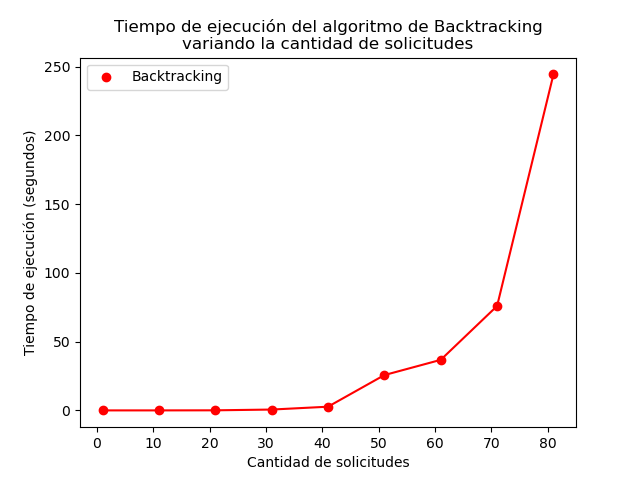
\includegraphics[width=\textwidth]{img/medicion_t_backtracking_var_m.png}
        \caption{Backtracking: Medición de tiempos variando $m$.}
        \label{fig:medicion_t_backtracking_var_m}
    \end{minipage}\hfill
    \begin{minipage}{0.45\textwidth}
        \centering
        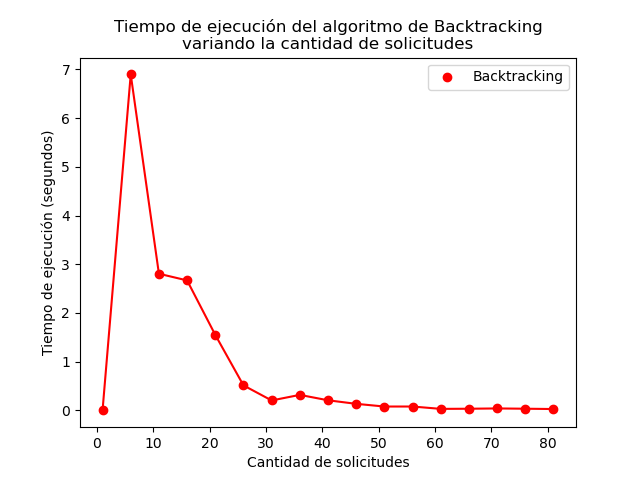
\includegraphics[width=\textwidth]{img/medicion_t_backtracking_var_b.png}
        \caption{Backtracking: Medición de tiempos variando $b$.}
        \label{fig:medicion_t_backtracking_var_b}
    \end{minipage}
\end{figure}

Por otro lado, el algoritmo de Programación Lineal Entera, contrario a lo esperado, presenta una gráfica más cercana a una función lineal (figs. \ref{fig:medicion_t_pl_var_m} y \ref{fig:medicion_t_pl_var_b}), asemejandose en tiempo de ejecución con el algorítmo de Programación Lineal Continua. Esto se debe a las optimizaciones implementadas en la librería \texttt{pulp} utilizada para su ejecución, las cuales reducen significativamente su tiempo de ejecución en comparación con su complejidad teórica. Es importante mencionar que la visualización de una curva exponencial en este algoritmo solo ocurre en situaciones donde las optimizaciones no influyen de manera considerable.

\begin{figure}[h]
    \centering
    \begin{minipage}{0.45\textwidth}
        \centering
        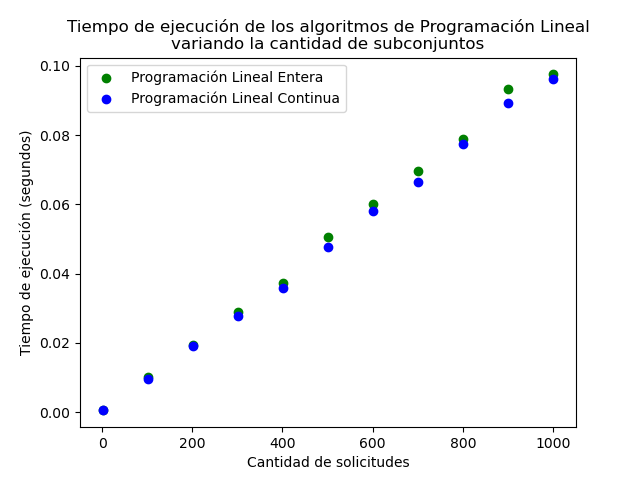
\includegraphics[width=\textwidth]{img/medicion_t_pl_var_m.png}
        \caption{Programación Lineal: Medición de tiempos variando $m$.}
        \label{fig:medicion_t_pl_var_m}
    \end{minipage}\hfill
    \begin{minipage}{0.45\textwidth}
        \centering
        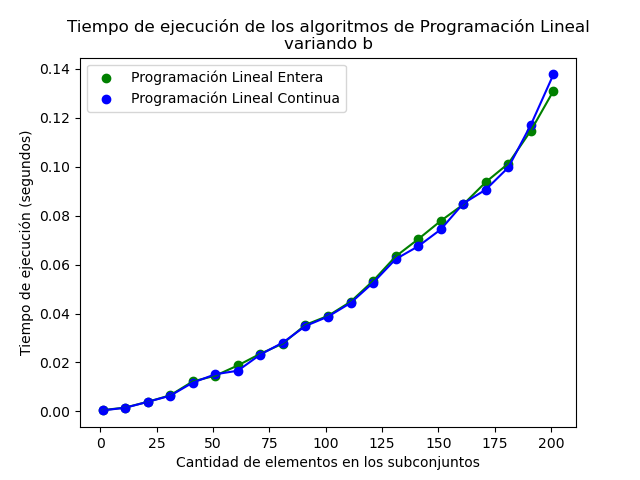
\includegraphics[width=\textwidth]{img/medicion_t_pl_var_b.png}
        \caption{Programación Lineal: Medición de tiempos variando $b$.}
        \label{fig:medicion_t_pl_var_b}
    \end{minipage}
\end{figure}

Por otro lado, podemos observar que la curva de Programación Lineal Continua se asemeja a una curva polinómica. De forma similar que en el caso de PLE, a pesar de que su cota teórica es un polinomio de grado $9$, en la gráfica se puede observar una tendencia lineal. Esto es debido a las diversas optimizaciones que la bilbioteca implementa y la escala de la medición.

En el siguiente gráfico, se ilustra el grado de aproximación, variando $b$ (fig. \label{medicion-plc-var-b}) y manteniendola constante (fig. \label{medicion-plc-cons-b}). Para poder corroborar nuestra cota máxima de aproximación, hicimos variar el parámetro $b$ en un intervalo $\left[25,30\right]$. Como en la gráfica se puede observar que la peor aproximación es $NUM_MAX$, luego se comprueba que la cota máxima es efectivamente en cada escenario es $b-1$.

Por otra parte, al examinar los algoritmos que emplean la estrategia de diseño Greedy, se evidencia que ambos siguen una tendencia polinomial. En el primer gráfico (fig. \ref{fig:medicion_t_greedy_var_m}), se observa una tendencia lineal. Esto se debe a que la variable $b$ permanece constante para cada escenario, variando únicamente la cantidad de subconjuntos ($m$). En contraste, a medida que se aumenta la cantidad de subconjuntos, se puede visualizar su tendencia polinómica no lineal, evidenciando la cota teórica (fig. \ref{fig:medicion_t_greedy_var_b}).

\begin{figure}[h]
    \centering
    \begin{minipage}{0.45\textwidth}
        \centering
        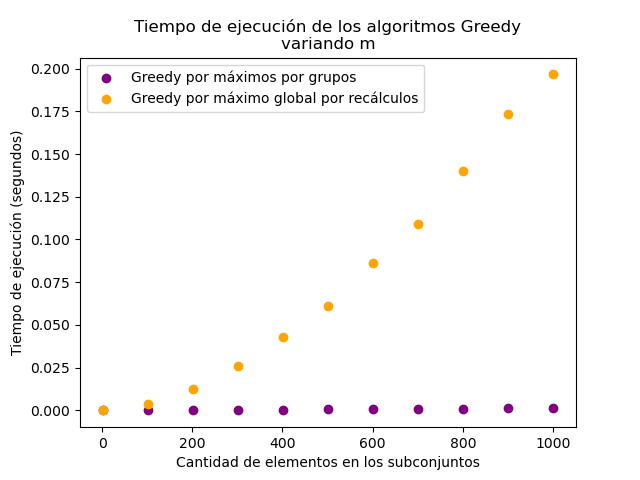
\includegraphics[width=\textwidth]{img/medicion_t_greedy_var_m.png}
        \caption{Greedy: Medición de tiempos variando $m$.}
        \label{fig:medicion_t_greedy_var_m}
    \end{minipage}\hfill
    \begin{minipage}{0.45\textwidth}
        \centering
        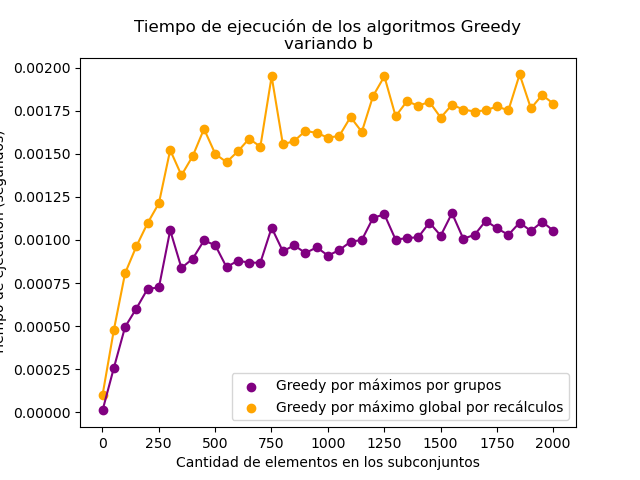
\includegraphics[width=\textwidth]{img/medicion_t_greedy_var_b.png}
        \caption{Greedy: Medición de tiempos variando $n$.}
        \label{fig:medicion_t_greedy_var_b}
    \end{minipage}
\end{figure}

Asimismo, se destaca una marcada diferencia en los tiempos de ejecución entre el algoritmo Greedy Máximo por Grupo y el algoritmo Greedy Máximo Global con Recálculo (figs. \ref{fig:medicion_r_greedy_var_m} y \ref{fig:medicion_r_greedy_var_b}). El primero muestra una ejecución significativamente más rápida en todos los escenarios comparado con el segundo. Sin embargo, al analizar las soluciones obtenidas, se evidencia que el algoritmo Greedy Máximo Global se acerca más a la solución óptima en todos los casos estudiados.

\begin{figure}[h]
    \centering
    \begin{minipage}{0.45\textwidth}
        \centering
        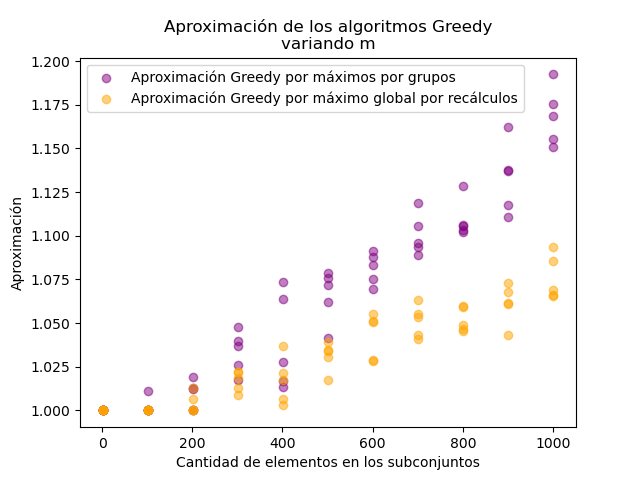
\includegraphics[width=\textwidth]{img/medicion_r_greedy_var_m.png}
        \caption{Greedy: Medición de tiempos variando $m$.}
        \label{fig:medicion_r_greedy_var_m}
    \end{minipage}\hfill
    \begin{minipage}{0.45\textwidth}
        \centering
        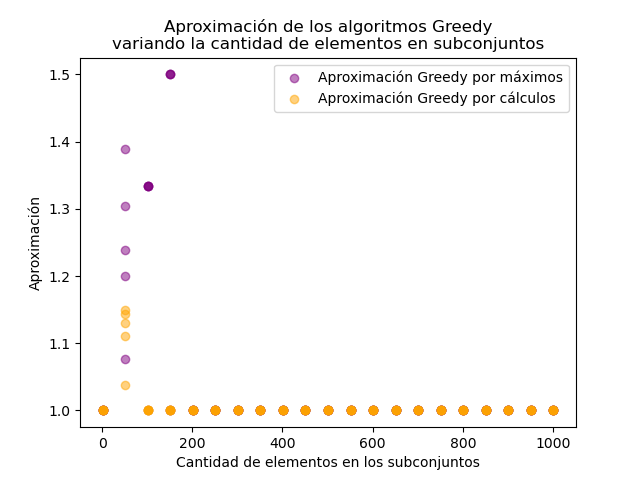
\includegraphics[width=\textwidth]{img/medicion_r_greedy_var_b.png}
        \caption{Greedy: Medición de tiempos variando $n$.}
        \label{fig:medicion_r_greedy_var_b}
    \end{minipage}
\end{figure}

Es interesante observar como el factor de aproximación $r(A)=\frac{A(I)}{z(I)}$ varía respecto a $m$ y a $b$. Para valores $b$ pequeños constantes, que es donde los dos algorítmos Greedy tienden a performar peor, no se aprecia una tendencia clara respecto a la variación de $m$ (fig. \ref{fig:medicion_r_greedy_var_m}). Sin embargo, con $m$ constante, se puede observar una tendencia inversamente proporcional entre $r(A)$ y $b$ (fig. \ref{fig:medicion_r_greedy_var_b}). Esto se debe a que, con grupos más grandes, la probabilidad de que un elemento pertenezca a más de un grupo es mayor, llegando al punto de que exista uno o varios jugadores en la intersección de todos los conjuntos. Ambos algoritmos greedy obtienen siempre la solución óptima en este caso, por lo que $\lim\limits_{b \rightarrow \infty}r(A)=1$.

\begin{figure}[h]
    \centering
    \begin{minipage}{0.45\textwidth}
        \centering
        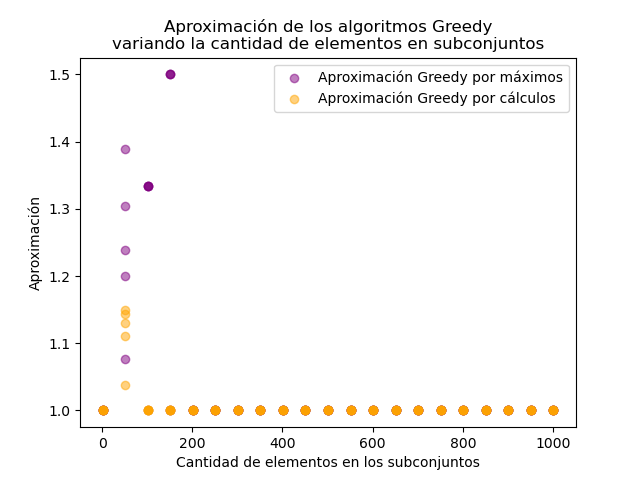
\includegraphics[width=\textwidth]{img/medicion_r_greedy_var_b.png}
        \caption{Greedy: Relación entre $r(A)$ y $b$ para $m$ constante.}
        \label{fig:medicion_r_greedy_var_b}
    \end{minipage}\hfill
    \begin{minipage}{0.45\textwidth}
        \centering
        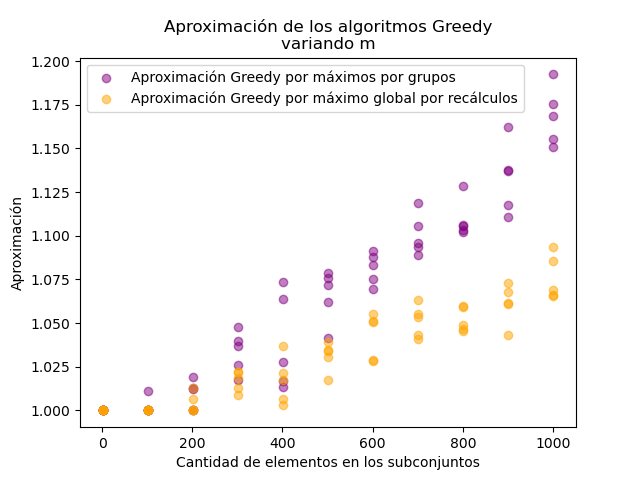
\includegraphics[width=\textwidth]{img/medicion_r_greedy_var_m.png}
        \caption{Greedy: Relación entre $r(A)$ y $m$ para $b$ constante.}
        \label{fig:medicion_r_greedy_var_m}
    \end{minipage}
\end{figure}

Esta divergencia plantea una dificultad al momento de decidir cuál enfoque es más adecuado. Por un lado, el algoritmo por grupo se destaca por su eficiencia temporal, ofreciendo tiempos de ejecución notoriamente inferiores y, por otro lado, el enfoque global muestra una mayor aproximación a la solución óptima.

!!! INSERTAR GRAFICOS !!!

% \begin{figure}[H]
%     \centering
%     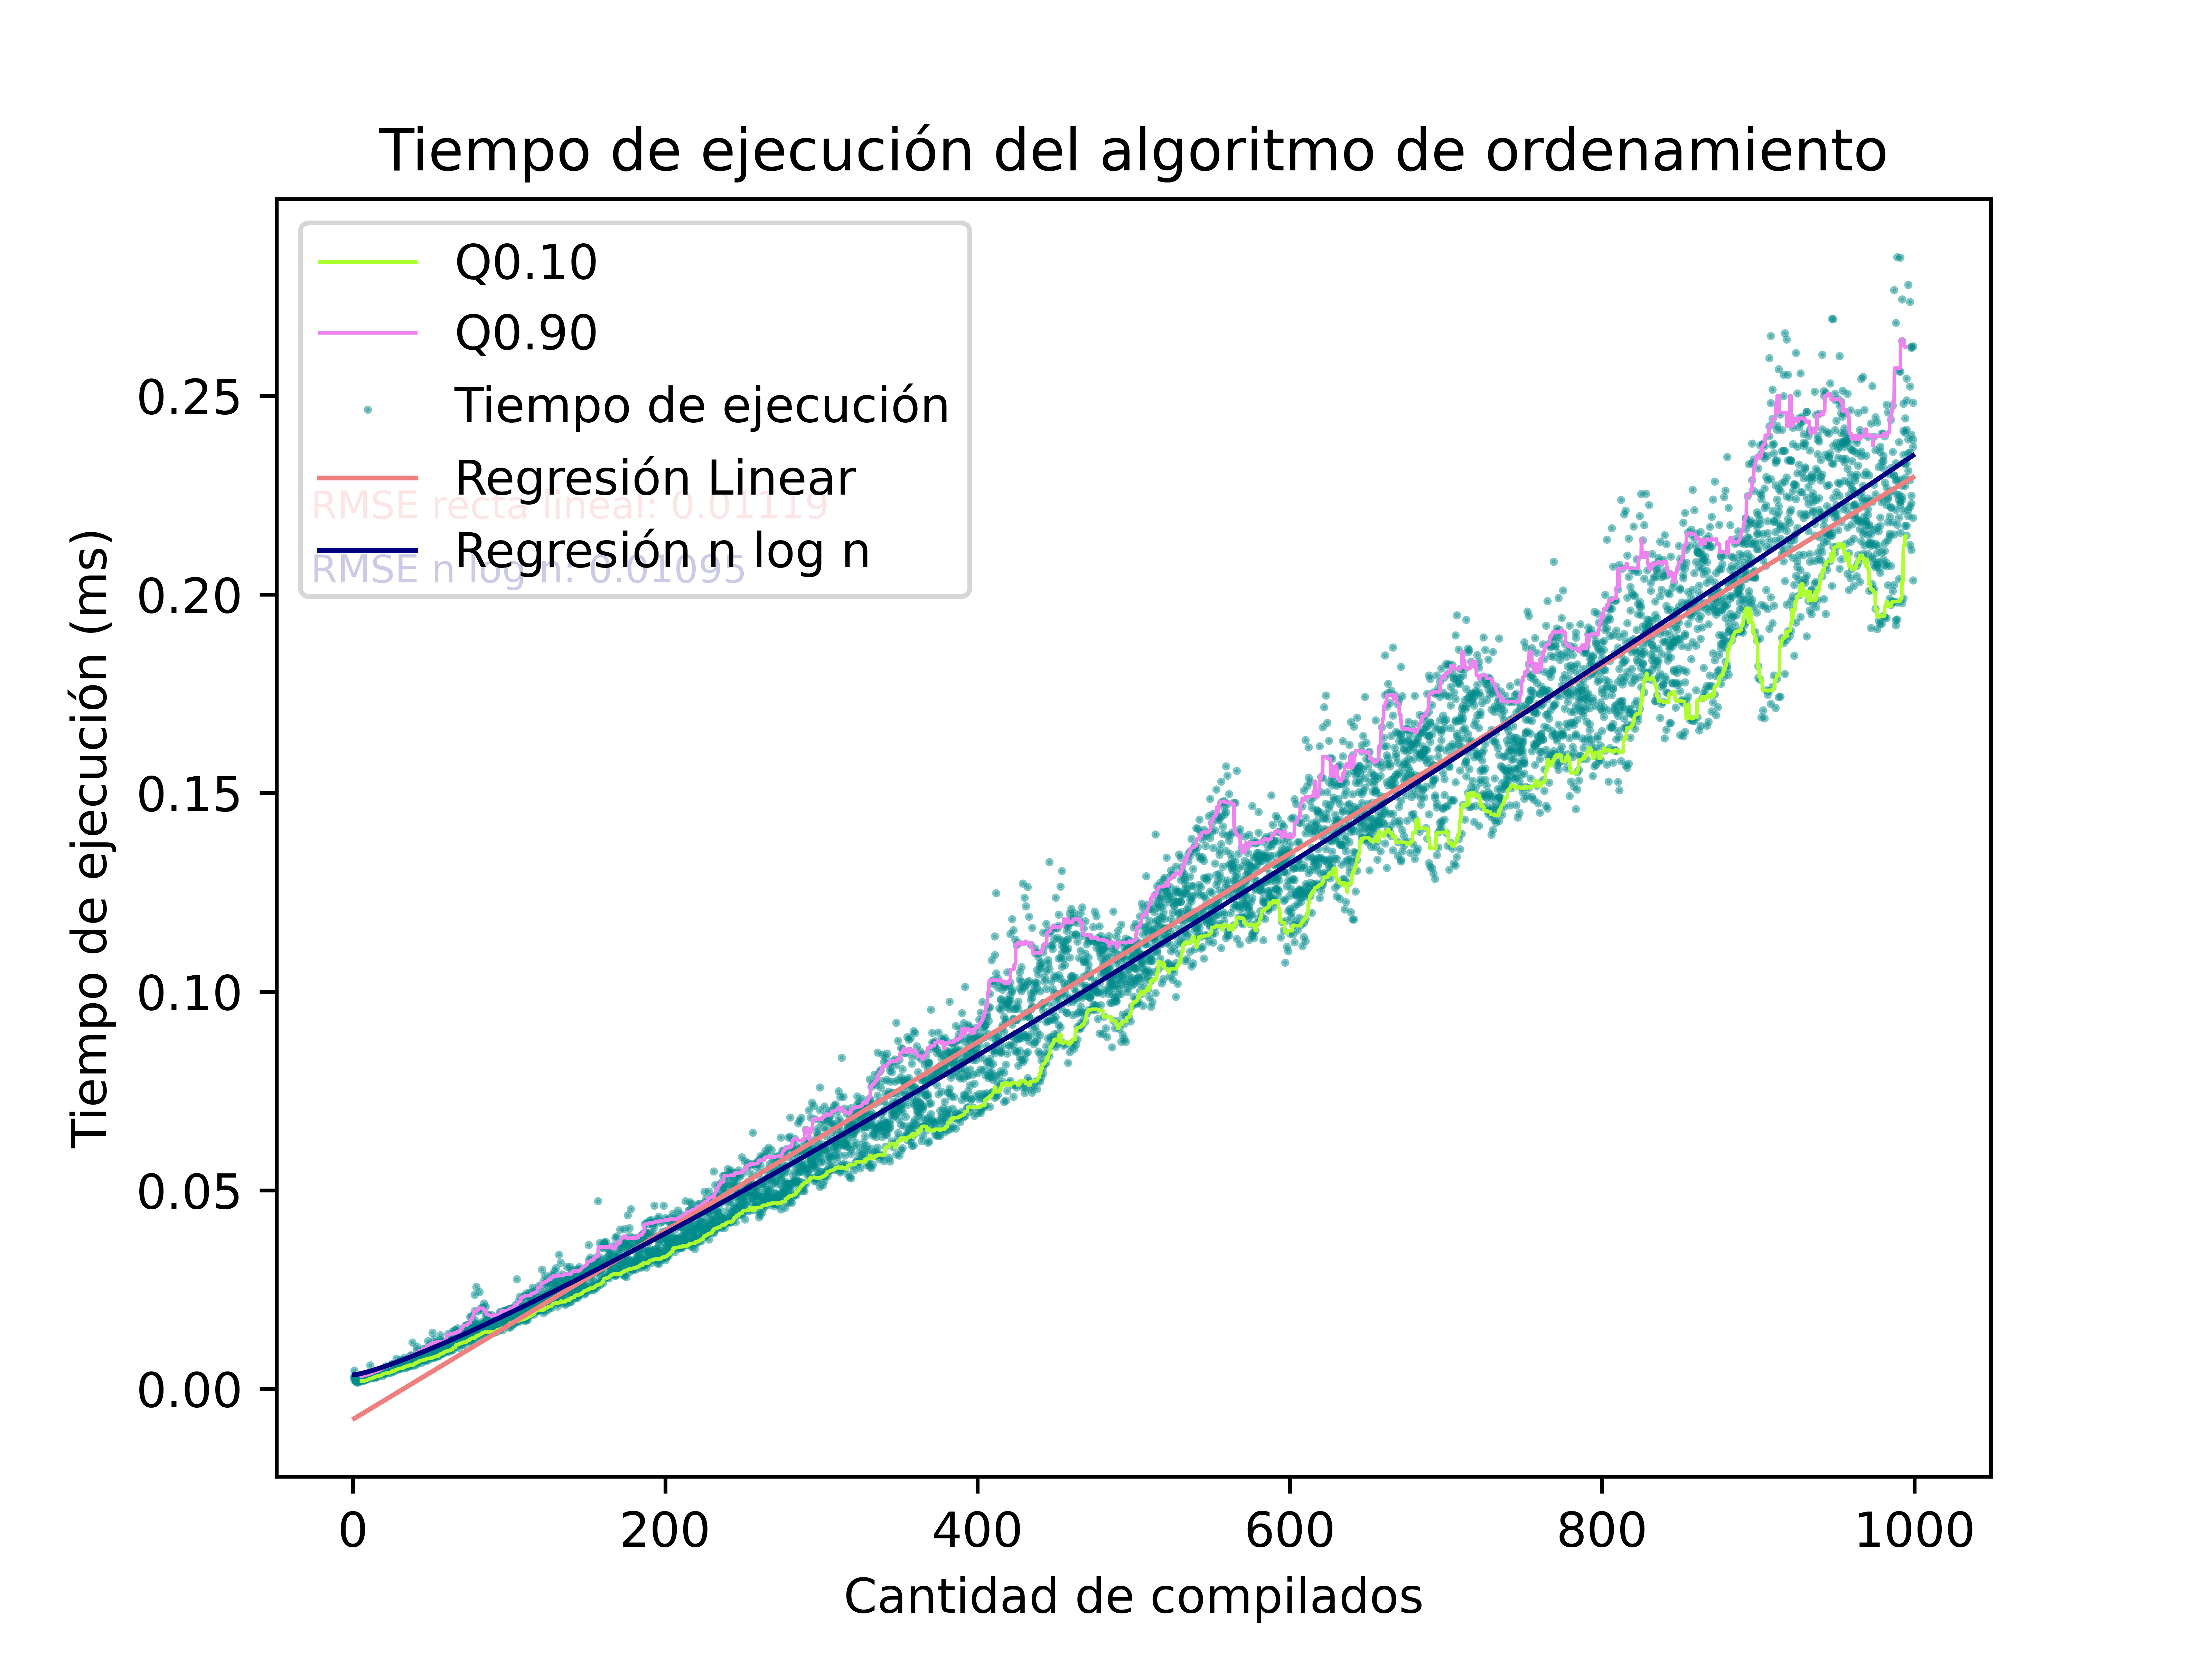
\includegraphics[width=0.8\textwidth]{img/tiempos_valores_bajos_puntos.png}
%     \caption{Tendencia de la complejidad algoritmica para $n$ pequeños.}
%     \label{fig:tiempos_valores_bajos_puntos}
% \end{figure}

% \begin{figure}[H]
%     \centering
%     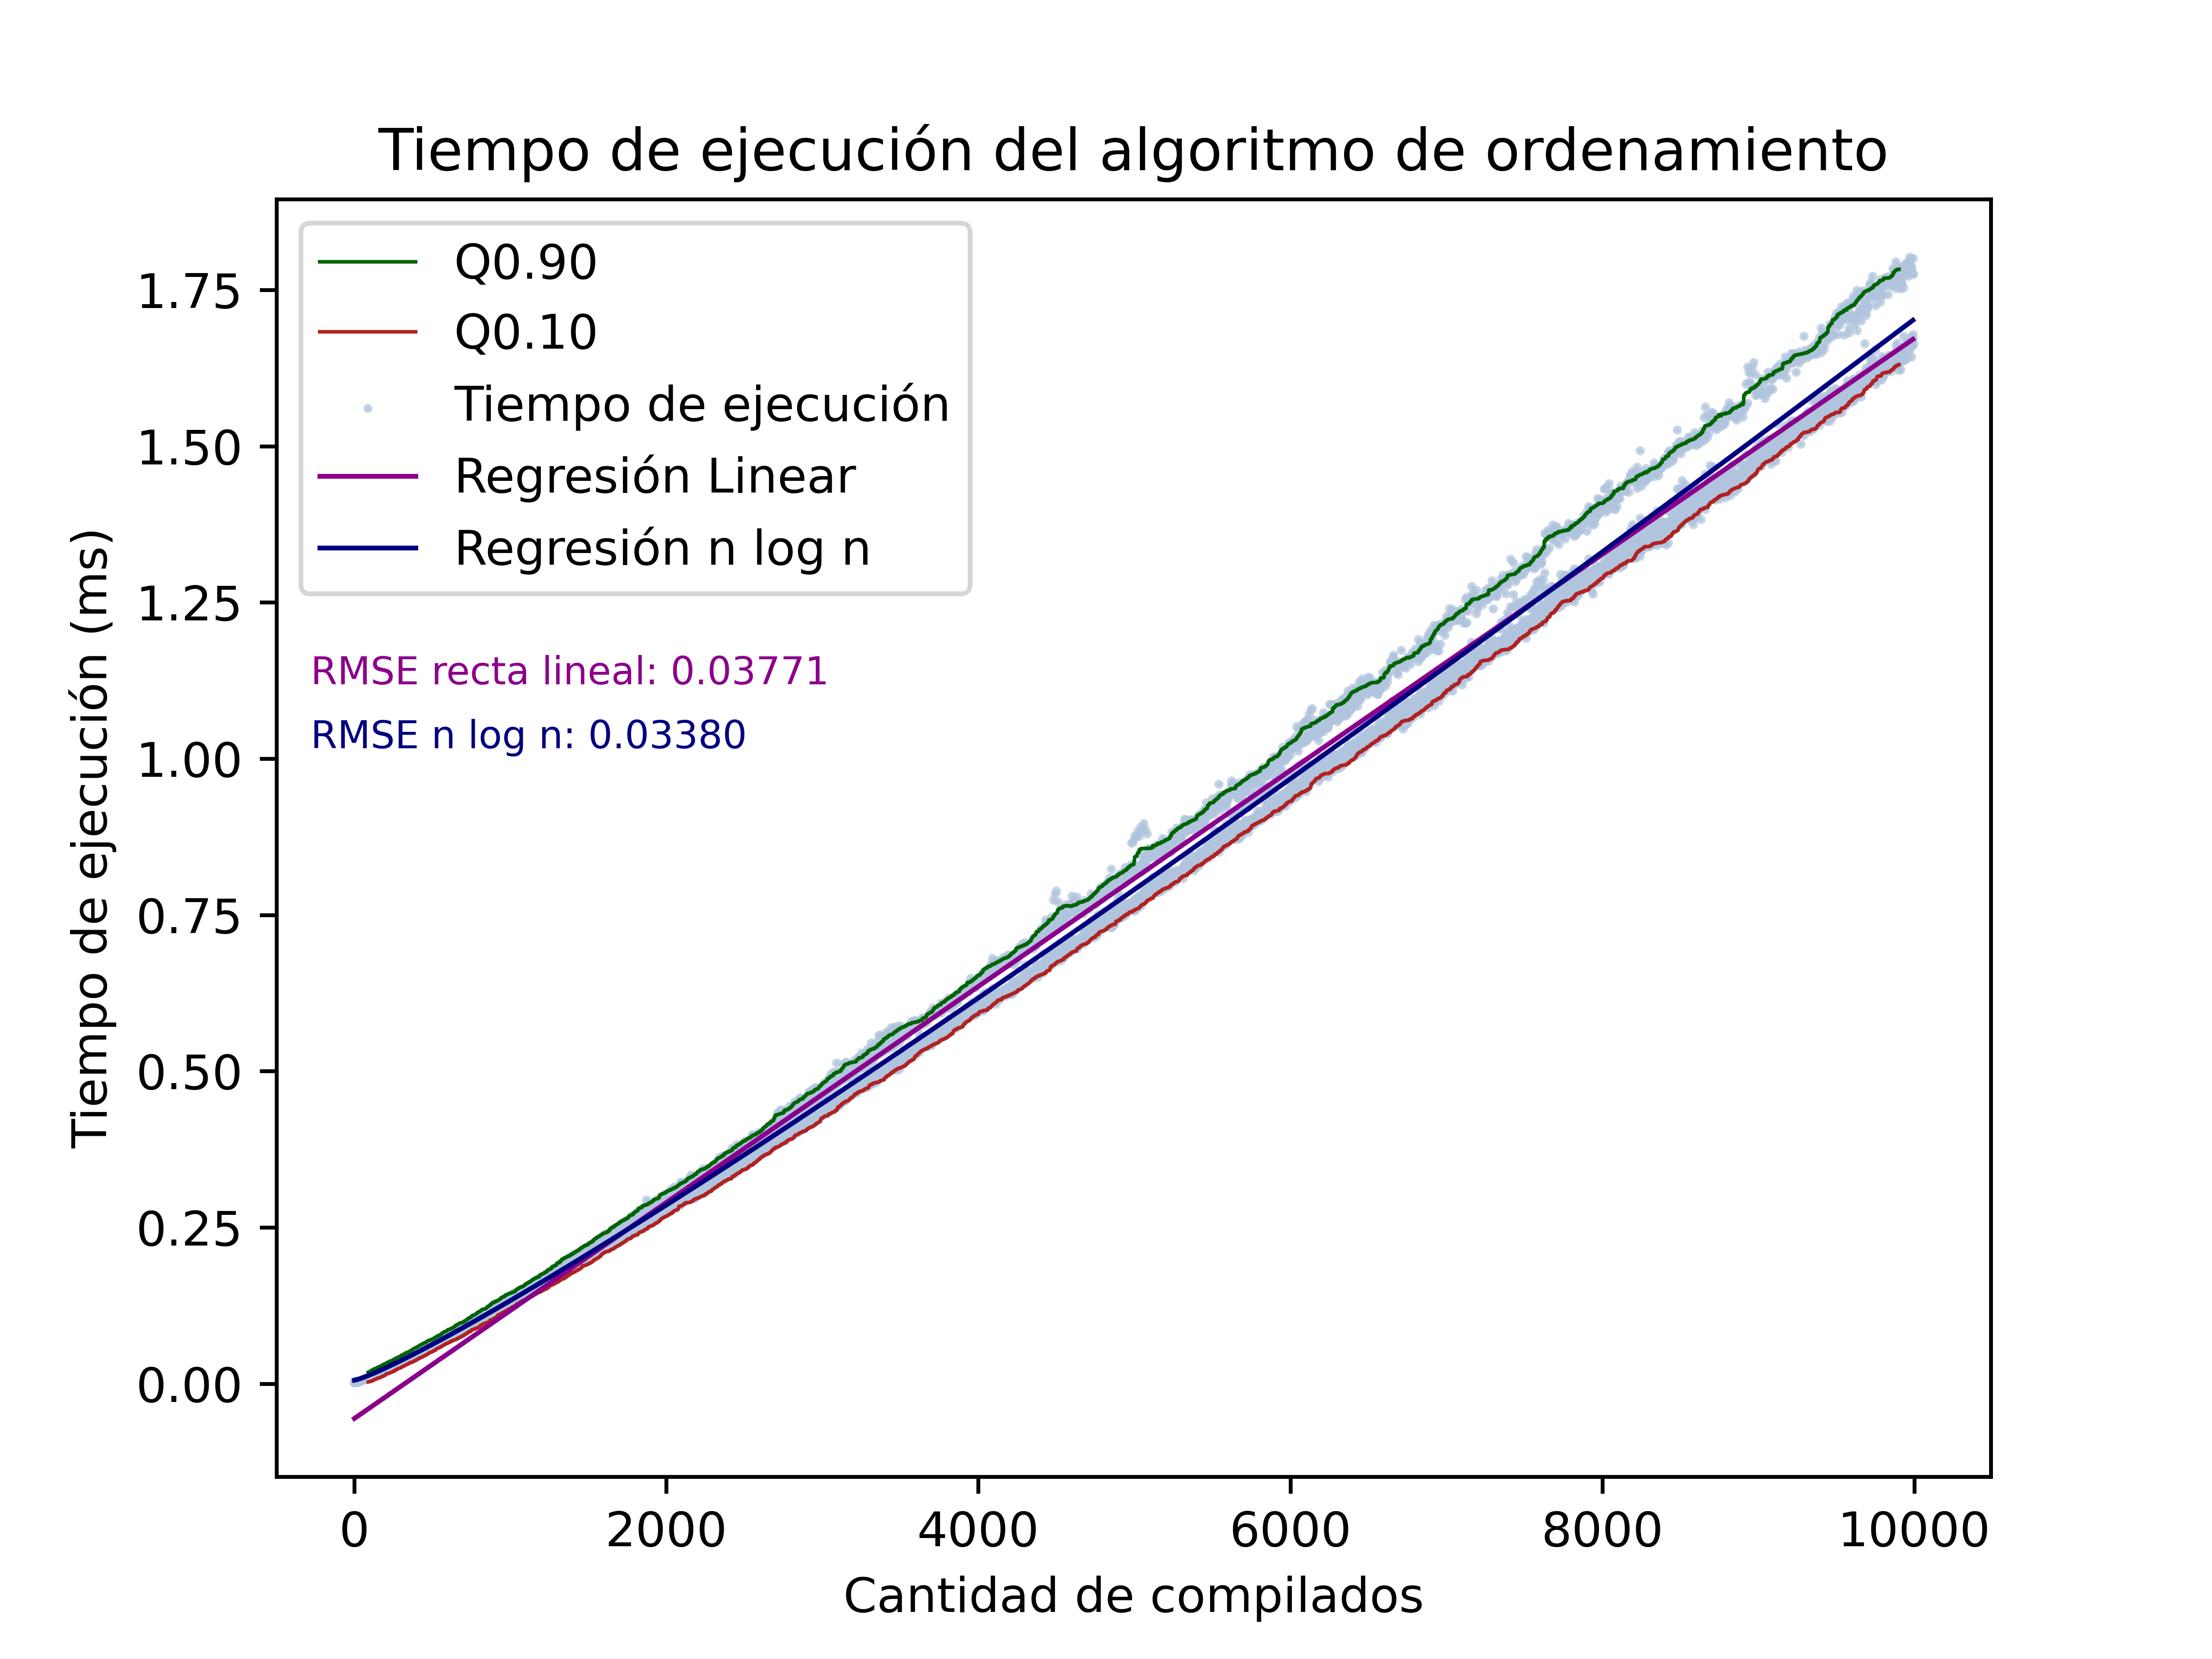
\includegraphics[width=0.8\textwidth]{img/tiempos_valores_altos_puntos.png}
%     \caption{Tendencia de la complejidad algoritmica para $n$ grandes.}
%     \label{fig:tiempos_valores_altos_puntos}
% \end{figure}
